
%(BEGIN_QUESTION)
% Copyright 2008, Tony R. Kuphaldt, released under the Creative Commons Attribution License (v 1.0)
% This means you may do almost anything with this work of mine, so long as you give me proper credit

Three-phase motors and generators alike are manufactured in two basic forms: {\it Wye} (Y) and {\it Delta} ($\Delta$):

$$\includegraphics[width=15.5cm]{i03258x01.eps}$$

Mark in the above diagrams where the following electrical quantities would be measured (hint: each coil shown in the diagram is called a {\it phase} winding, and each conductor connecting the motor or generator to something else in the three-phase system is called a {\it line}):

\begin{itemize}
\item{} Phase voltage
\item{} Line voltage
\vskip 5pt
\item{} Phase current
\item{} Line current
\end{itemize}

In which circuit (Wye or Delta) are the phase and line currents equal?  In which circuit (Wye or Delta) are the phase and line voltages equal?  Explain both answers, in terms that anyone with a basic knowledge of electricity could understand (i.e. using the properties of {\it series} and {\it parallel} connections).  Where phase and line quantities are {\it un}equal, determine which is larger.

\underbar{file i03258}
%(END_QUESTION)





%(BEGIN_ANSWER)

$$\includegraphics[width=15.5cm]{i03258x02.eps}$$

\begin{itemize}
\goodbreak
\item{} {\bf Wye configuration} 
\item{} $I_{phase} = I_{line}$
\item{} $V_{phase} < V_{line}$ 
\end{itemize}

\begin{itemize}
\goodbreak
\item{} {\bf Delta configuration} 
\item{} $V_{phase} = V_{line}$ 
\item{} $I_{phase} < I_{line}$
\end{itemize}

%(END_ANSWER)





%(BEGIN_NOTES)


%INDEX% Electronics review: 3-phase electrical power 

%(END_NOTES)


